\title{Esercitazione 5 23/04/2020}\newline
\textbf{link} \href{https://web.microsoftstream.com/video/e80c852f-1851-42f7-9a73-dfb6b8d85ee9}{Clicca qui} [... praticamente solo audio]
\section{Esercitazione V}
\url{../esercitazione5/pdf/05-Esercizio 2.pdf}\newline
\url{../esercitazione5/pdf/05-Statica01.pdf}\newline
\url{../esercitazione5/pdf/ese_5_notes.pdf}
\subsection{Ripasso sulle equazioni cardinali della statica}
\textbf{Equazioni cardinali della statica} per l'equilibrio statico:
\begin{itemize}
    \item \textbf{Equilibrio alla traslazione}:\[
        \sum \vec{F} = 0 
    \]
    la somma di tutte le forze applicate deve essere nulla, queste forze si suddividono in forze attive e reattive:
    \[
        \sum_j \vec{F}_j + \sum_r \vec{R}_{v,r} = 0
    \]
    Questa equazione è in forma vettoriale e quindi la si può proiettare nel piano $XY$ per ottenere due equazioni.
    \item La somma di tutti i momenti rispetto a un polo $O$ deve essere nullo.
    \[
        \sum \vec{M}_O = 0
    \]
    Possiamo riscrivere la somma della risultante di forze e coppie applicate al corpo rigido e della risultante di forze e coppie di reazioni vincolari:
    \[
        \sum_j (P_j - O) \land \vec{F}_j + \sum_k \vec{C}_k + \sum_r (P_r-O) \land \vec{R}_{v,r} + \sum _s \vec{C}_{v,s} = 0
    \]
\end{itemize}
\subsection{Ripasso sul momento di una forza}
Il momento di una forza è la capacità di una forza di indurre una torsione su un corpo rigido ed è definito come
\[
    \vec{M}_O = (P-O) \land \vec{F}
\]
\subsection{Ripasso sulle azioni interne}
Isolando una sezione di un corpo rigido si introducono tre tipi di azioni:
\begin{itemize}
    \item azioni assiali;
    \item azioni di taglio;
    \item momento flettente;
\end{itemize}
Per convenzione si assumono positive le azioni interne in questi versi:\newline
[immagine dagli appunti del prof]
\begin{center}
    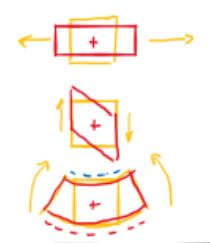
\includegraphics[height=4cm]{../esercitazione5/img1.JPG}
\end{center}
Ricordiamo, inoltre, anche se fuori tema, che i momenti si prendono positivi in senso antiorario.
\newline
\newline
Nel disegnare i diagrammi sui corpi rigidi delle azioni interne, per il momento flettente va disegnato positivo nel verso delle fibbre tese (non contratte). Per gli altri due, cioè azioni assiali e di taglio, è indifferente, basta ricordarsi di scrivere il segno.